% Template: LaTeX file for ICMC 2011 papers, with hyper-references
%
% derived from the DAFx-06 templates
% derived from the ICMC 2009 templates by Steve Beck
% and then derived from the ICMC 2010 template
% 1) Please compile using latex or pdflatex.
% 2) Please use figures in vectorial format (.pdf); .png or .jpg are working otherwise 
% 3) Please use the "papertitle" and "pdfauthor" commands defined below

%------------------------------------------------------------------------------------------
\documentclass[twoside,10pt,a4paper]{article}
\usepackage{icmc2011,amssymb,amsmath} 
\usepackage[utf8]{inputenc}
\usepackage{url}
\usepackage{verbatim}
\usepackage{mathptmx} 

%\setcounter{page}{1}

%____________________________________________________________
\sloppy
\newenvironment{contentsmall}	{\small}

\newenvironment{gmncode}		{\vspace{-2mm}\small\verbatim}{\endverbatim\vspace{-2mm}}


\newcommand{\GMN}			{\emph{Guido Music Notation}}
\newcommand{\Guido}		{\textsc{Guido}}
\newcommand{\GAR}			{GuidoAR}
%\newcommand{\syntax}[1]	{\vspace{-3mm} \small #1}
\newcommand{\code}[1]		{{\small \texttt{#1}}}
\newcommand{\gtag}[1]		{$\backslash$\code{#1}}
%\newcommand{\todo}[1]		{{\\ \hspace*{-8mm} \textbf{Todo:} \texttt{#1}}}
\newcommand{\rulenum}[1]	{\textbf{#1}}
\newcommand{\oend}			{\emph{opened-end}}
\newcommand{\obeg}			{\emph{opened-begin}}
\newcommand{\obegend}		{\emph{opened-begin-end}}
\newcommand{\codeindent}	{\\ \hspace*{9mm}}

%____________________________________________________________
%  !  !  !  !  !  !  !  !  !  !  !  ! user defined variables  !  !  !  !  !  !  !  !  !  !  !  !  !  !
%==== set the title ====
\def\papertitle{Scores Level Composition based on the Guido Music Notation}
%\def\papertitle{}	%-- should be empty for the submission anyway!

%==== 1st submission: author name and affiliation are empty for anonymous submission ====
\def\paperauthorA{} 
\affiliation{}{}


%==== final submission: author name and affiliation ====
%---- uncomment 1 to 4 lines, for 1 to 4 authors
\def\paperauthorA{D. Fober}
\def\paperauthorB{Y. Orlarey}
\def\paperauthorC{S. Letz}
\def\paperauthorD{}

%%---- set correspnding affiliation data for...
%%-- 1 author
%\affiliation{\paperauthorA}
%  {School\\ Department, City, Country \\ {\tt \href{mailto:email@domain.icmc}{email@domain.icmc}}}

%%-- 2 authors with same affiliation
\affiliation{\paperauthorA, \paperauthorB, \paperauthorC}
  {Grame\\ Centre national de crétaion musicale, Lyon, France \\ {\tt \href{mailto:fober@grame.fr}{fober@grame.fr}}}

%-- 2 authors with different affiliations
%\twoaffiliations{\paperauthorA}{School\\ Department}
%  {\paperauthorB}{Company\\ Address}

%%-- 3 authors with different affiliations
%\threeaffiliations{\paperauthorA}{School A\\ Department X}
%  {\paperauthorB}{Company\\ Address}
%  {\paperauthorC}{School B\\ Department Y}

%%-- 4 authors with different affiliations
%\fouraffiliations{\paperauthorA}{School A\\ Department X}
%  {\paperauthorB}{Company\\ Address}
%  {\paperauthorC}{School B\\ Department Y}
%  {\paperauthorD}{School C\\ Department Z}

%  ^  ^  ^  ^  ^  ^  ^  ^  ^  ^ user defined variables  ^  ^  ^  ^  ^  ^  ^  ^  ^  ^  ^  ^ 
%------------------------------------------------------------------------------------------

%%-- if using .ps or .eps figure files, they will be converted on the fly
%%-- RMK: for faster LaTeX runs, use it only once after adding new \includegraphics[]{} cmds
%\usepackage{epstopdf}	 

%---- the hyperref package must be last to properly work
\usepackage[pdftex,
       pdftitle={\papertitle},
	pdfauthor={\paperauthorA},
	colorlinks=false,bookmarksnumbered,pdfstartview=XYZ]{hyperref}
%\pdfcompresslevel=9
\usepackage[pdftex]{graphicx}	% for compatible graphics with hyperref
\usepackage[figure,table]{hypcap}	% corrects the hyper-anchor of figures/tables

\title{\papertitle}

%------------------------------------------------------------------------------------------
\begin{document}

\DeclareGraphicsExtensions{.png,.jpg,.pdf} % used graphic file format for pdflatex
    
\maketitle

\begin{abstract}
Based on the Guido Music Notation format, we have developed tools for music score \emph{"composition"} (in the etymological sense), i.e. operators that take scores both as target and arguments of high level transformations, applicable for example to the time domain (e.g. cutting the head or the tail of a score) or to the structural domains (e.g. putting scores in sequence or in parallel). 
Providing these operations at score level is particularly convenient to express music ideas and to compose these ideas in an homogeneous representation space. However, scores level composition gives raise to a set of issues related to the music notation consistency. This paper introduces the \Guido\ Music Notation format, presents the score composition operations, the notation issues and a proposal to solve them.
\end{abstract}


%----------------------------------------------------------------
\section{Introduction}\label{sec:intro}
%----------------------------------------------------------------
The \Guido\ Music Notation format [GMN] \cite{hoos98} has been designed by H. Hoos and K. Hamel more than ten years ago. It is a general purpose formal language for representing score level music in a platform independent plain text and human readable way. It is based on a conceptually simple but powerful formalism: its design concentrates on general musical concepts (as opposed to graphical characteristics). A key feature of the \Guido\ design is adequacy which means that simple musical concepts are represented in a simple way and only complex notions require complex representations.

Based on the GMN language, the \Guido\ Library \cite{daudin09a,Fober:04b} provides a powerful score layout engine that differentiates from the compiler solutions for music notation \cite{lilypond03,musixtex} by its ability to be embedded into standalone applications, and by its fast and efficient rendering engine, making the system usable in \emph{real-time} for simple music scores.

Based on the combination of the \Guido\ language and engine, score level composition operators have been designed, providing time or pitch transformations, composition in sequence or in parallel, etc.
Developing score level composition operators provides an homogeneous way to write scores and to manipulate them while remaining at a high music description level. Moreover, the design allows to use scores both as target and as arguments of the operations, enforcing the notation level metaphor.

However, applied at score level, these operations raise a set of issues related to the music notation consistency. We propose a simple typology of the music notation elements and a set of rules based on this typology to enforce the music notation coherence.

The next section introduces the \Guido\ Music Notation format, followed by a presentation of the score composition operations, the related notation problems and the proposed solutions, including a language extension to handle reversibility issues.

%----------------------------------------------------------------
\section{The Guido Music Notation format}
%----------------------------------------------------------------

\subsection{Basic concepts}
%----------------------------------------------------------------
Basic \Guido\ notation covers the representation of notes, rests, accidentals, single and multi-voiced music and the most common concepts from conventional music notation such as clefs, meter, key, slurs, ties, beaming, stem directions, etc.
Notes are specified by their name \code{(a b c d e f g h)}, optional accidentals ('\#' and '\&' for sharp and flat), an optional octave number and an optional duration. \\
Duration is specified in one of the forms: 
\begin{gmncode} 
   '*'enum'/'denom dotting
   '*'enum dotting 
   '/'denom dotting
\end{gmncode} 
\noindent where $enum$ and $denom$ are positive integers and $dotting$ is either empty, '.', or '..'. When $enum$ or $denom$ is omitted, it is assumed to be 1. The duration represents a whole note fractional.

When omitted, optional note description parts are assumed to be equal to the previous specification before in the current sequence.

Chords are described using comma separated notes enclosed in brackets e.g \code{\{c, e, g\}}

\subsection{\Guido\ tags}
%----------------------------------------------------------------
Tags are used to represent additional musical information, such as slurs, clefs, keys, etc. A basic tag has one of the forms:
\begin{gmncode} 
   \tagname 
   \tagname<param-list>
\end{gmncode}
\noindent where \code{param-list} is a list of string or numerical arguments, separated by commas (','). In addition, a tag may have a time range and be applied to a series of notes (e.g. slurs, ties, etc.); the corresponding forms are:
\begin{gmncode} 
   \tagname(note-series)
   \tagname<param-list>(note-series)
\end{gmncode} 

The following GMN code illustrates the concision of the notation; figure \ref{ex1} represents the corresponding \Guido\ engine output. 
\begin{gmncode} 
  [ \meter<"4/4"> \key<-2> c d e& f/8 g ]
\end{gmncode} 

\begin{figure}[h]
	\centering 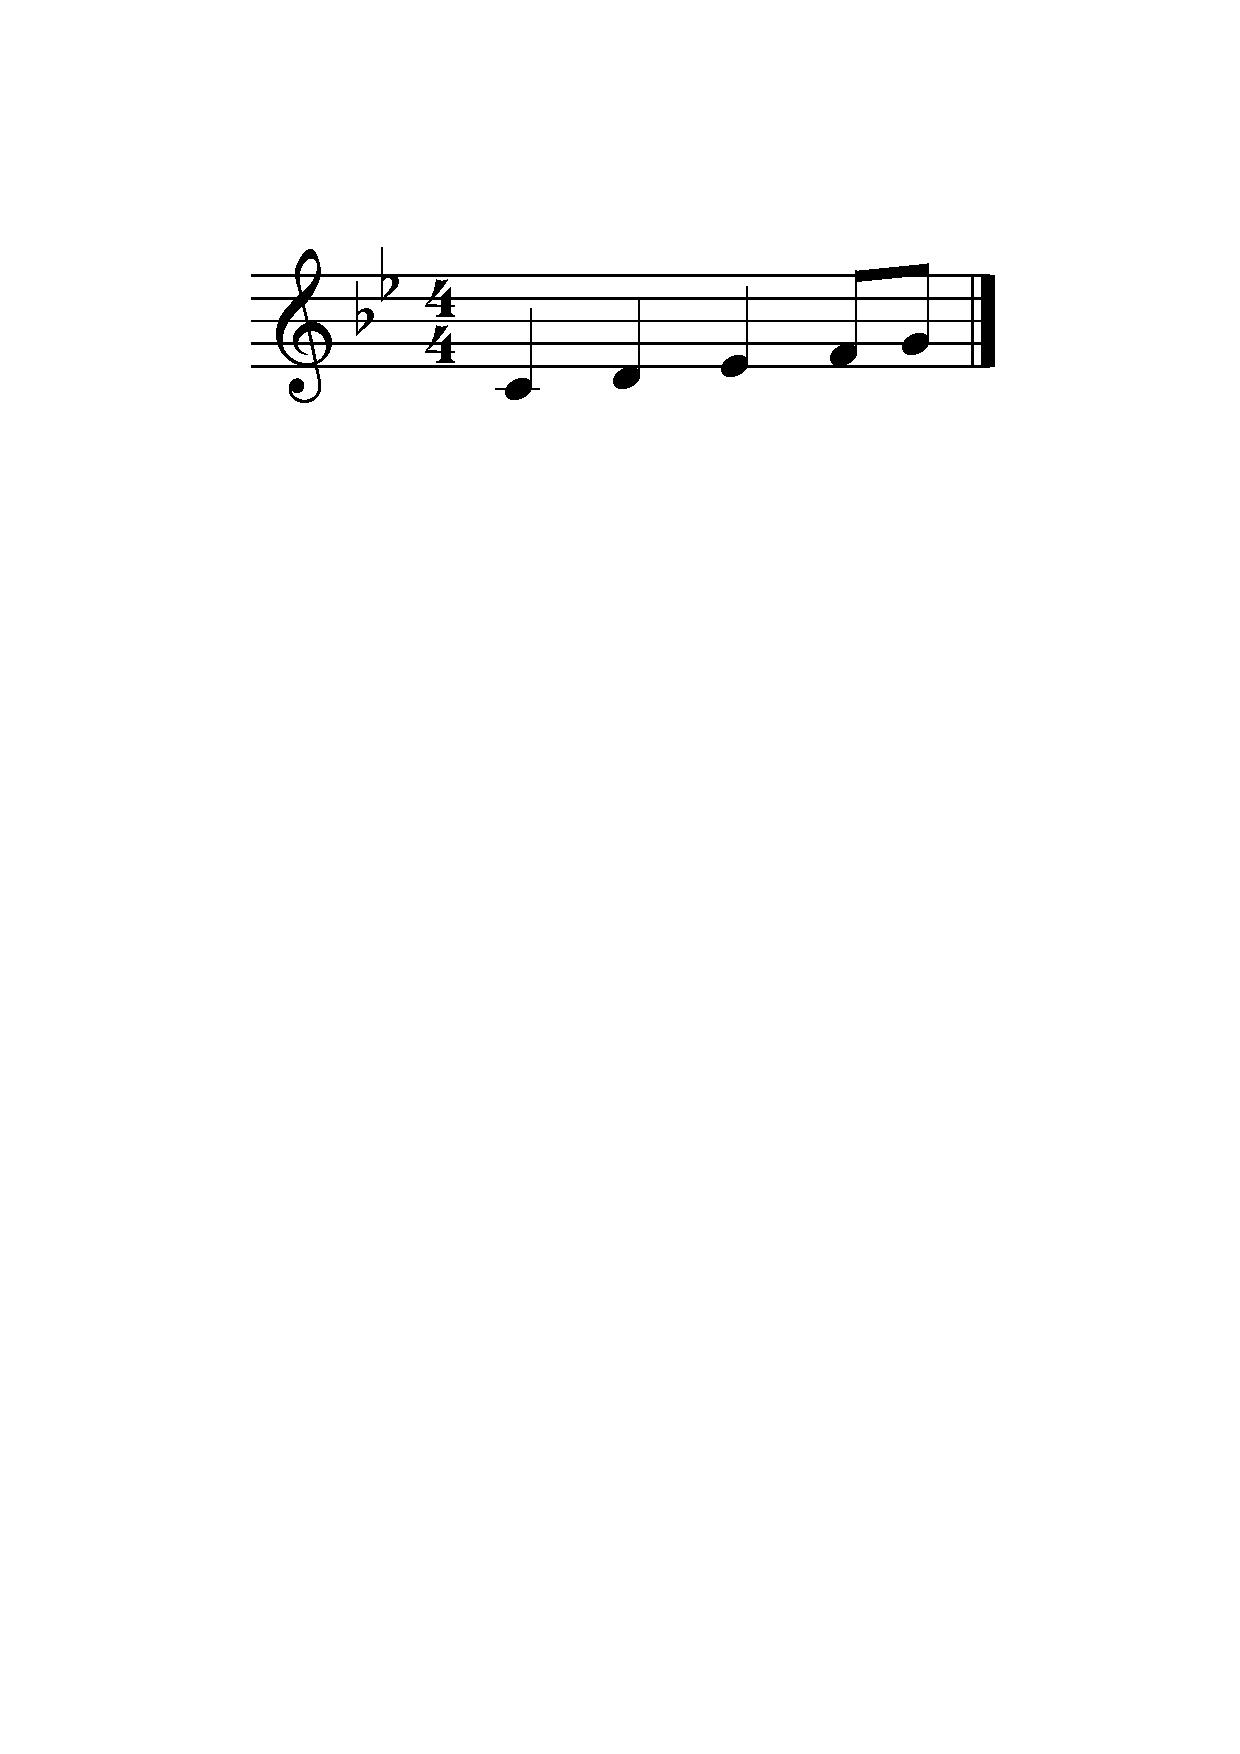
\includegraphics[width=47mm]{imgs/ex1}
 \caption{A simple GMN example}
 \label{ex1}
\end{figure}

\subsection{Notes sequences and segments}
%----------------------------------------------------------------
A note sequence is of the form \verb+[tagged-notes]+ where \code{tagged-notes} is a series of notes, tags, and tagged ranges separated by spaces. Note sequences represent single-voiced scores.
Note segments represent multi-voiced scores; they are denoted by \verb+{seq-list}+ where \code{seq-list} is a list of note sequences separated by commas as shown by the example below (figure \ref{fig:voices}):
\codeindent\code{ \{ [ e g f ], [ a e a ] \} }
\begin{figure}[h]
	\centering 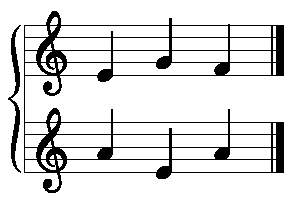
\includegraphics[width=32mm]{rsrc/voices}
 \caption{A multi-voices example}
 \label{fig:voices}
\end{figure}


\subsection{Advanced \Guido.}
%----------------------------------------------------------------
The advanced \Guido\ specification extends basic \Guido\ with more tags and more tags parameters, giving more control over the score layout.
For example, it introduces tags parameters like $dx$ and $dy$ for fine positioning of the score elements, notes and rests format specifications, staff assignments, etc. 
%Below is an example of advanced guido with the corresponding output (figure \ref{advex}).
%
%\begin{gmncode} 
%{
% [
%  \barFormat<"system">
%  \staff<1> \stemsUp \meter<"2/4"> 
%  \intens<"p", dx=1hs,dy=-7hs>
%  \beam(g2/32 e/16 c*3/32) c/8 
%  \beam(\noteFormat<dx=-0.9hs>(a1/16) c2 f) 
%  \beam(g/32 d/16 h1*3/32) d2/8 
%  \beam(h1/16 d2 g)],
% [\staff<1>\stemsDown g1/8 e
%  f/16 \noteFormat<dx=0.8hs>(g) f a a/8 e 
%  f/16 g f e],
% [\staff<2> \meter<"2/4"> 
%  \stemsUp a0 f h c1],
% [\staff<2> \stemsDown c0 d g {d, a}]
%}
%\end{gmncode} 
%
%\begin{figure}[h]
%	\centering 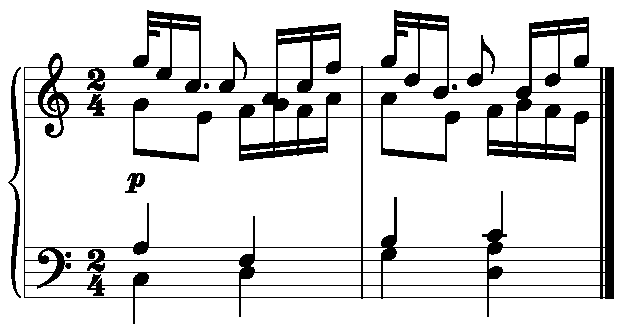
\includegraphics[width=0.85\columnwidth]{rsrc/4voices}
% \caption{An advanced Guido example}
% \label{advex}
%\end{figure}


%----------------------------------------------------------------
\section{Composing Music Scores}
%----------------------------------------------------------------

Since \Guido\ is a concise textual format, it seems natural to use operations commonly applied to text, like cut, copy and paste, text concatenation, etc. Thus the first idea with the score level operations was based on textual manipulation, extended to music specific operations.


%----------------------------------------------------------------
\subsection{Operations}
Score level operations are given by table \ref{operations}. These operations are available as library API calls, as command line tools, or using a graphic environment named \Guido Calculus. Almost all of the operations take a GMN score and a value parameter as input and produce a GMN score as output. The value parameter can be taken from another GMN score:
for example, the \code{top} operation cuts the bottom voices of a score after a given voice number; when using a score as parameter, the voice number is taken from the score voices count.

All the operations concentrate on the transformed dimension (pitch, time), without modifying user defined elements or trying to interfere with the automatic layout of the \Guido\ Engine (that may add notation elements like clef, barlines). For example, the \emph{duration} operation recomputes the notes length but doesn't affect the time signature or the barlines. 
When two scores are put in parallel, the system preserves each voice time and key signatures, even when they don't match. The transposition operation is the only exception: it adds or modifies the key signature and selects the  simplest enharmonic diatonic transposition. 

The design allows all the operations to take place consistently at the notation level. Using the command line tools, series of transformations can be expressed as pipelining scores through operators e.g. \\
\hspace*{4mm} \code{head s1 s2 | par s2 | transpose "[ c ]" }



\begin{table*}[htdp]
\begin{center}
\begin{tabular}{rll}
\hline
operation & args		&	description \\
\hline
seq 	&	$s1\ s2$		& puts the scores $s1$ and $s2$ in sequence \\
par 	&	$s1\ s2$		& puts the scores $s1$ and $s2$ in parallel \\ 
rpar	&	$s1\ s2$		& puts the scores $s1$ and $s2$ in parallel, right aligned \\
top 	&	$s1\ [n\ | \ s2]$ 	& takes the $n$ top voices of $s1$; \\
		&	& when using a score $s2$ as parameter, $n$ is taken from $s2$ voices count \\
bottom 	&	$s1\ [n\ | \ s2]$ 	& takes the bottom voices of $s1$ after the voice $n$;  \\
		&	& when using a score $s2$ as parameter, $n$ is taken from $s2$ voices count \\
head	& 	$s1\ [d\ | \ s2]$	& takes the head of $s1$ up to the date $d$; \\
		& 	& when using a score $s2$ as parameter, $d$ is taken from $s2$ duration \\
evhead 	&	$s1\ [n\ | \ s2]$	& id. but on events basis i.e. the cut point is specified in $n$ events count; \\
		& 	& when using a score $s2$ as parameter, $n$ is taken from $s2$ events count \\
tail	&	$s1\ [d\ | \ s2]$ 	& takes the tail of a score after the date $d$; \\
		& 	& when using a score $s2$ as parameter, $d$ is taken from $s2$ duration \\
evtail 	&	$s1\ [n\ | \ s2]$ 	& id. but on events basis i.e. the cut point is specified in $n$ events count; \\
		& 	& when using a score $s2$ as parameter, $n$ is taken from $s2$ events count \\
transpose 	&	$s1\ [i\ | \ s2]$	& transposes $s1$ to an interval $i$; \\
			& 	& when using a score $s2$ as parameter, $i$ is computed as the difference between \\
			& 	& the first voice, first notes of $s1$ and $s2$ \\
duration 	&	$s1\ [d\ |\ r\ |\ s2]$	& stretches $s1$ to a duration $d$ or using a ratio $r$; \\
			& 	& when using a score $s2$ as parameter, $d$ is computed from $s2$ duration \\
applypitch 	&	$s1\ s2$	& applies the pitches of $s1$ to $s2$ in a loop \\
applyrythm 	&	$s1\ s2$	& applies the rhythm of $s1$ to $s2$ in a loop \\
\hline
\end{tabular}
\end{center}
\caption{Score level operations}
\label{operations}
\end{table*}

%----------------------------------------------------------------
\subsection{Notation issues}
\label{issues}
Actually, the score level composition functions operate on a memory representation of the music notation. But we'll illustrate the notation issues with the textual representation which is equivalent to the memory representation.

Let's take an example with the \code{tail} operation applied to the following simple score: 
\codeindent \code{[\gtag{clef}<"f"> c d e c]}\\
A raw cut of the score after 2 notes would give \code{[e\ c]}, removing the clef information and potentially leading to unexpected results (figure \ref{fig:tail}).
\begin{figure}[h]
	\centering 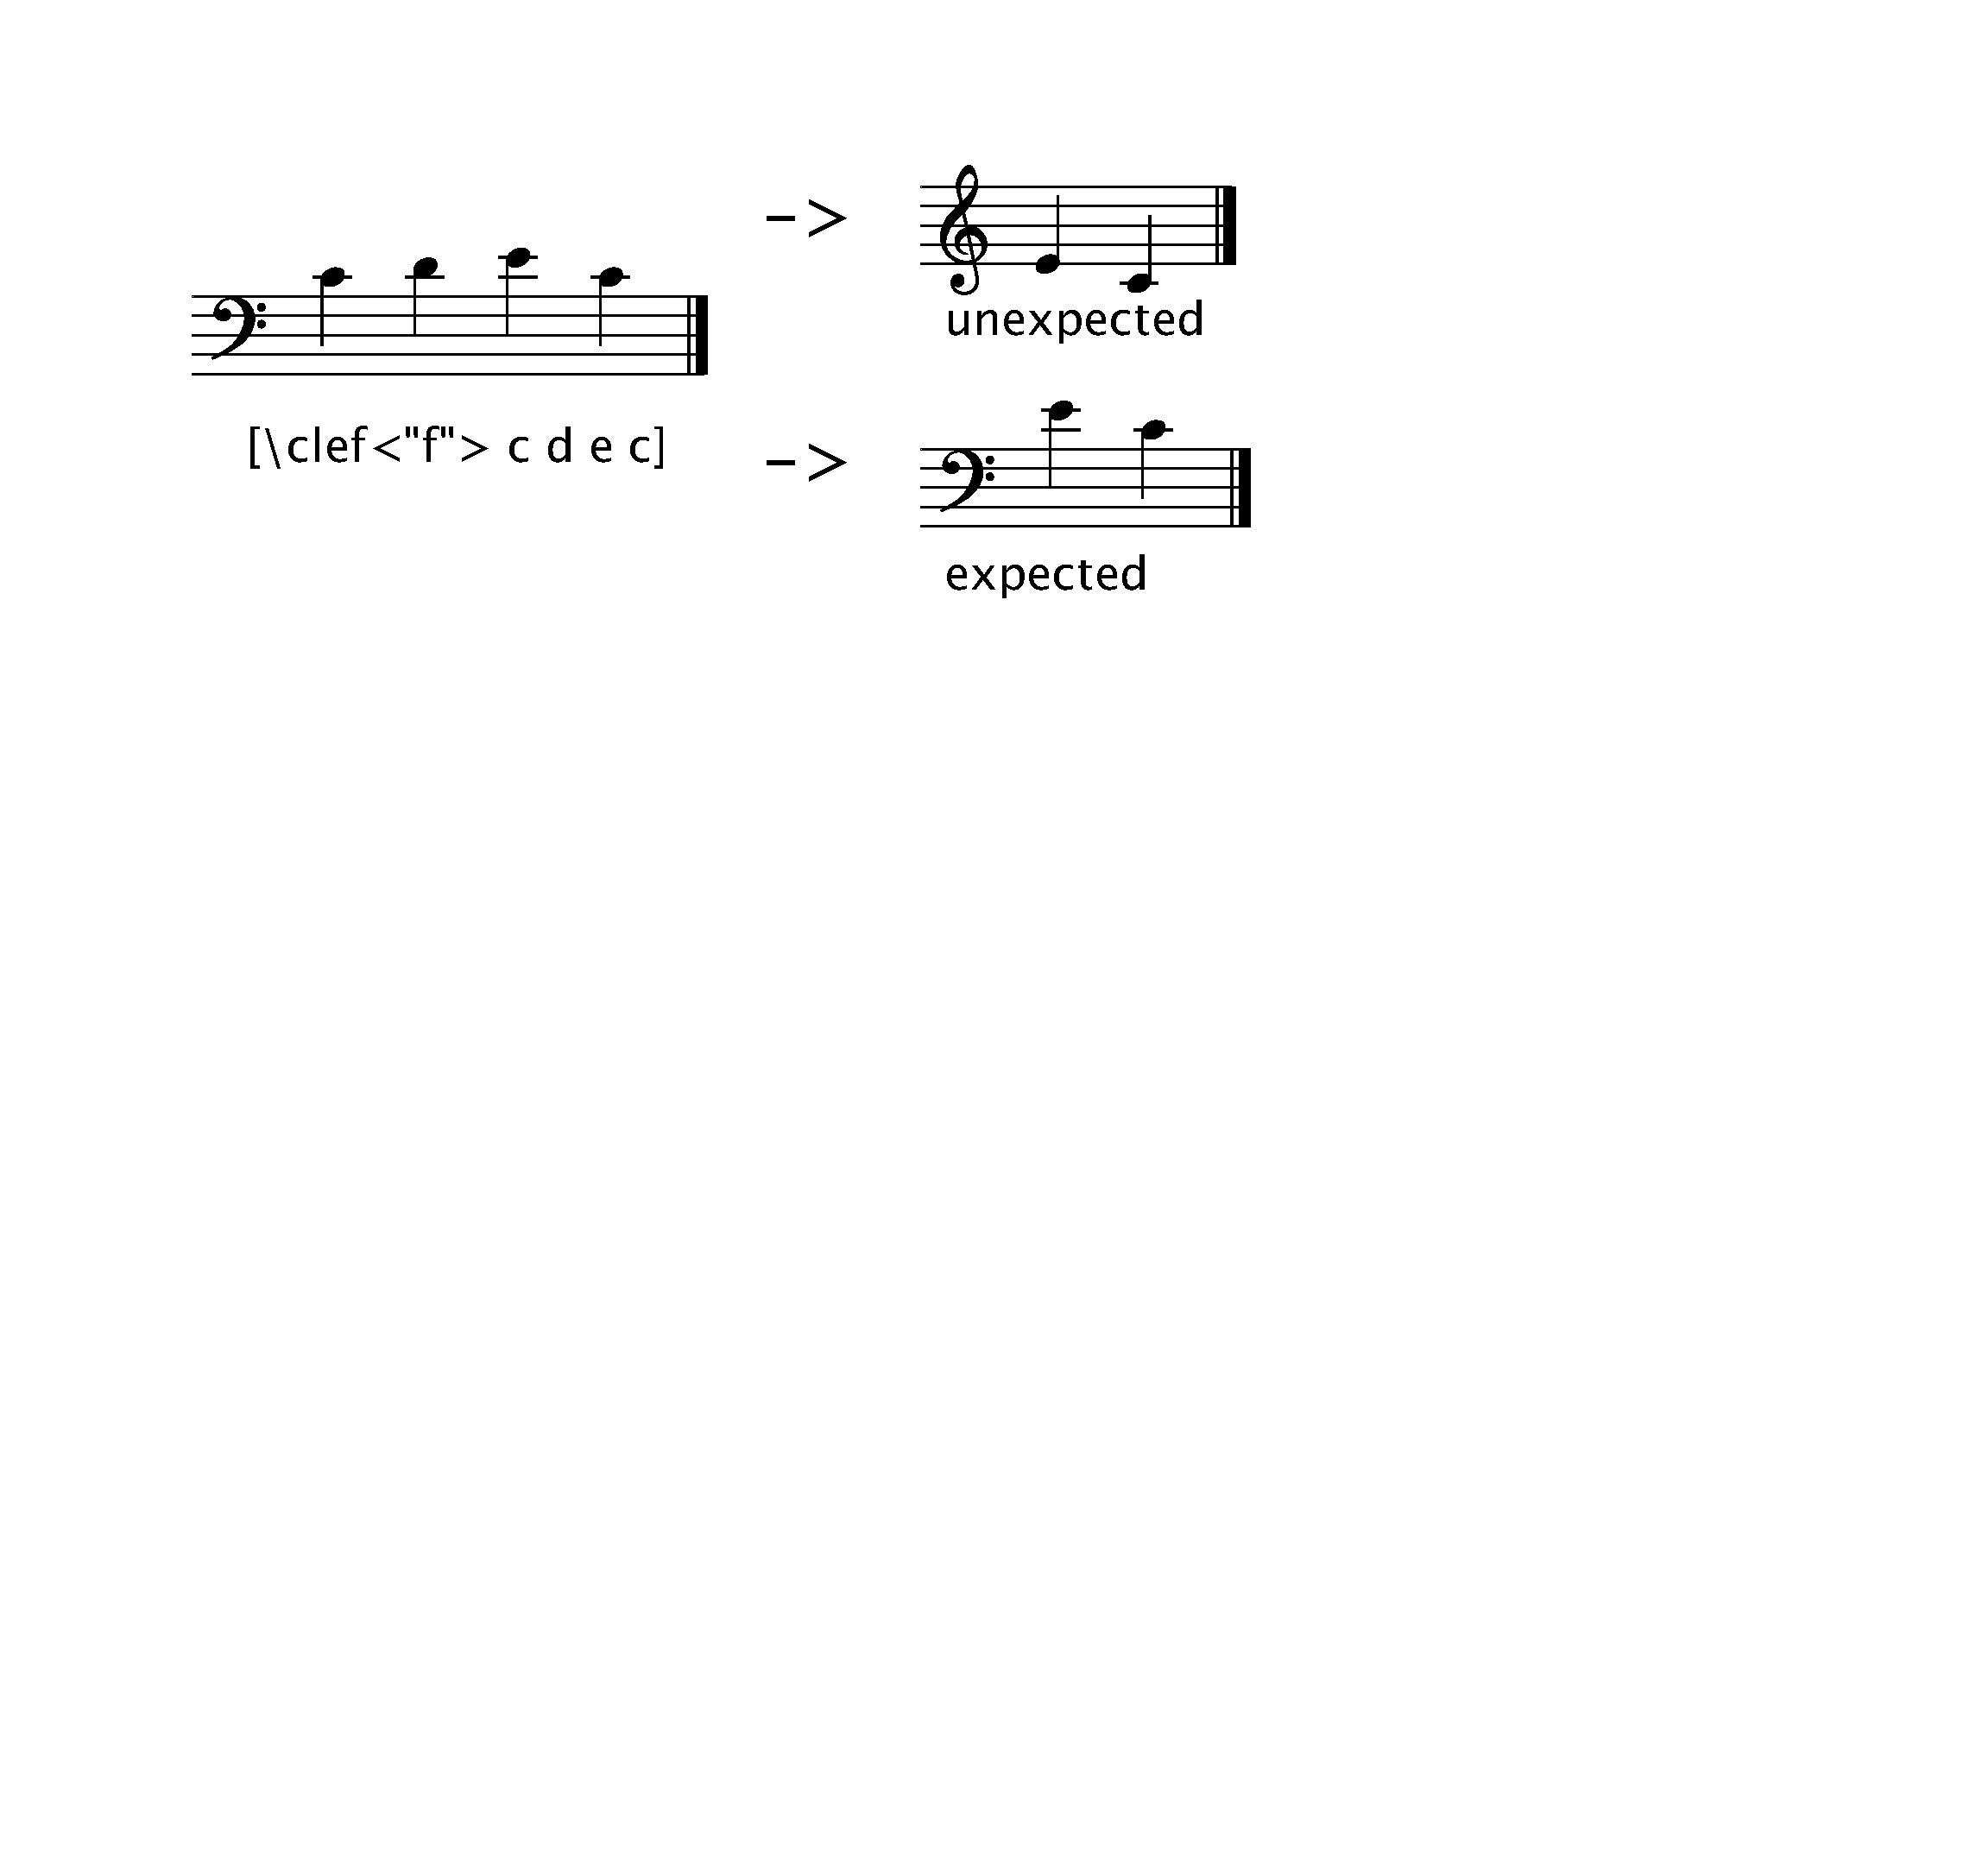
\includegraphics[width=60mm]{imgs/tail}
 \caption{Tail operation consistency}
 \label{fig:tail}
\end{figure}

Here is another example with the \code{seq} operation: a raw sequence of 
\hspace{2mm} \code{[\gtag{clef}<"g"> c d]} \\
and \hspace{14.5mm}\code{[\gtag{clef}<"g"> e c]} \\
would give \hspace{3.1mm} \code{[\gtag{clef}<"g"> c d \gtag{clef}<"g"> e c ]} 
where the clef repetition (figure \ref{fig:seq2}) is useless and blurs the reading.
\begin{figure}[h]
	\centering 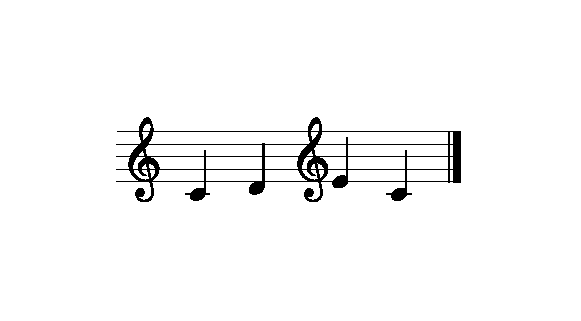
\includegraphics[width=40mm]{imgs/seq2}
 \caption{A raw sequence operation}
 \label{fig:seq2}
\end{figure}

Some operations may also result in syntactically incorrect results. Consider the following code:
\codeindent \code{[g \gtag{slur}(f e) c]} \\
slicing the score in 2 parts after \code{f} would result in 
\codeindent \textbf{a)}\ \ \code{[g \gtag{slur}(f]} \ \  and \textbf{b)} \ \  \code{[e) c]} \\
i.e. with uncompleted range tags. We'll use the terms \oend\ tags to refer the a) form and \obeg\ tags for the b) form.

These simple examples illustrate the problem and there are many more cases where the music notation consistency has to be preserved across score level operations.

%----------------------------------------------------------------
\section{Music Notation consistency}
%----------------------------------------------------------------

In order to solve the notation issues, we propose a simple typology of the notation elements regarding their time extent and a set of rules defining adequate consistency policies according to the operations and the elements type.

%----------------------------------------------------------------
\subsection{Notation elements time extent}

The GMN format makes a distinction between \emph{position} tags (e.g. \gtag{clef}, \gtag{meter}) and \emph{range} tags (e.g. \gtag{slur}, \gtag{beam}). Position tags are simple notations marks at a given time position while range tags have an explicit time extent: the duration of the enclosed notes. 
However, this distinction is not sufficient to cover the time status of the elements: many of the position tags have an implicit time duration and generally, they last up to the next similar notation or to the end of the score. For example, a dynamic lasts to the next dynamic or the end of the score.
\begin{table*}[htdp]
\begin{center}
\begin{tabular}{cll}
time extent & description & sample \\
\hline
explicit 	& duration is explicit from the notation	& slurs, cresc. \\
implicit 	& element lasts to the next similar element or to the end of the score		& meter, dynamics, key \\
others 		& structure control			& coda, da capo, repeats\\
	- 		& formatting instructions		& new line, new page \\
	- 		& misc. notations	& breath mark, bar \\
\hline
\end{tabular}
\end{center}
\caption{Typology of notation elements.}
\label{types}
\end{table*}

Table \ref{types} presents a simple typology of the music notation elements, mainly grounded on their time extent.
Based on this typology, provisions have to be made when:
\begin{itemize}
\item computing the beginning of a score:  
\begin{description}
	\item[1)] the pending explicit time extent elements must be properly opened (i.e. \obeg\ tags, see section \ref{issues})
	\item[2)] the current implicit time extent elements must be recalled,
\end{description}
\item computing the end of a score: 
\begin{description}
	\item[3)] the explicit time extent elements must be properly closed (i.e. \oend\ tags)
\end{description}
\item putting scores in sequence: 
\begin{description}
	\item[4)] implicit time extent elements starting the second score must be skipped when they correspond to current existing elements.
\end{description}
\end{itemize}

%----------------------------------------------------------------
\subsection{Structure control issues} \label{sc}
Elements relevant to the \emph{others / structure control} time extent category may also give rise to inconsistent notation: a \emph{repeat begin} bar without \emph{repeat end}, a \emph{dal segno} without \emph{segno}, a \emph{da capo al fine} without \emph{fine}, etc. We introduce new rules to catch the repeat bar issue. Let's first define a \emph{pending} repeat end as the case of a voice with a repeat begin tag without matching repeat end.
\begin{itemize}
\item[\rulenum{5)}] when computing the end of a score, every \emph{pending} repeat end must be closed with a repeat end tag.
\item[\rulenum{6)}] from successive unmatched repeat begin tags, only the first one must be retained.
\item[\rulenum{7)}] from successive repeat end tags, only the last one must be retained.
\end{itemize}
No additional provision is made for the other structure control elements: possible inconsistencies are ignored but this choice preserves the operations reversibility.

%----------------------------------------------------------------
\subsection{Operations reversibility}\label{reverse}
The above rules solve most of the notation issues but they do not permit the operations to be reverted: consider a score including a slur, sliced in the middle of the slur and reverted by putting the parts back in sequence. The result will include two slurs (figure \ref{fig:rev}) due to the rules \rulenum{1)} and \rulenum{3)}  that enforce opening \obeg\ tags and closing \oend\ tags.
\begin{figure}[h]
	\centering 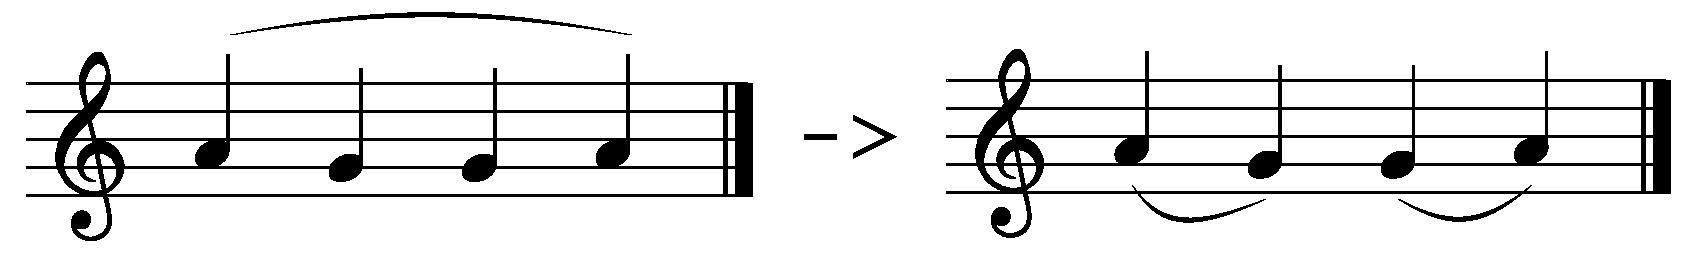
\includegraphics[width=80mm]{imgs/reverse}
 \caption{A score sliced and put back in sequence}
 \label{fig:rev}
\end{figure}

To solve the problem, we need the support of the GMN language and we introduce a new tag parameter, intended to keep the history of range tags and to denote \oend\ and/or \obeg\ ancestors.
The parameter has the form: 
\codeindent \code{open="type"} \\
where \code{type} is in [\code{begin}, \code{end,} \code{begin-end}], corresponding to \obeg, \oend, and \obegend\ ancestors.

Next, we introduce a new rule for score level operations. Let's first define \emph{adjacent} tags as tags placed on the same voice and that are not separated by any note or chord. Note that range tags are viewed as containers and thus, notes in the range do not separate tags.
\begin{itemize}
\item[\rulenum{8)}] \emph{adjacent} similar tags carrying an \code{open} parameter are mutually cancelled when the first one is \oend\ and the second one \obeg . 
\end{itemize}
For example, the application of this rule to the following score: 
\codeindent \code{[ \gtag{anytag}<open="end">(f g) 
 \codeindent \gtag{anytag}<open="begin">(f e) ]}\\
will give the score below:
\codeindent\code{[ \gtag{anytag}(f g f e) ]} 

Note that Advanced \Guido\ allows range tags to be expressed using a \code{Begin} and \code{End} format (e.g. \gtag{slurBegin}, \gtag{slurEnd} instead \gtag{slur(range)}). This format is handled similarly to regular range tags and the \code{open} parameter is also implemented for Begin/End tags.

%----------------------------------------------------------------
\section{Conclusion}
%----------------------------------------------------------------
Music notation is complex due to the large number of notation elements and to the heterogeneous status of these elements. The typology proposed in table \ref{types} is actually a simplification intended to cover the needs of score level operations but it is not representative of this complexity. However, it reflects the music notation semantic and could be reused with other score level music representation language. Thus apart for the reversibility rule that requires the support of the music representation language, all the other rules are independent from the GMN format and applicable in other contexts.

Score level operations could be very useful in the context of batch processing (e.g. voices separation from a conductor, excerpt extraction, etc.). The operations presented in table \ref{operations} support this kind of processing but they also open the door to a new approach of the music creative process. 


\bibliographystyle{IEEEtranS}
\bibliography{../guido} % requires file template.bib

\end{document}
